\chapter{Evaluation}\label{cha:evaluation}

In this chapter, we will discuss our evaluation with the goal of answering the research questions in \Cref{cha:author-extraction}.

Three typical metrics for assessing the performance of a sequence tagging task are \gls{precision}, \gls{recall}, and the \gls{f1 score}~\citep{councill2008parscit}.
Given a sequence of words where each word is assigned a label out of a set of labels $L$, \gls{precision} and \gls{recall} are defined as~\citep{goutte2005probabilistic}:
\begin{equation*}
  \textit{precision}(L)=\frac{TP(L)}{TP(L)+FP(L)}\hspace{4em}\textit{recall}(L)=\frac{TP(L)}{TP(L)+FN(L)}
\end{equation*}
Here, $TP(L)$, $FP(L)$, and $FN(L)$ stand for the number of True Positive, False Positive, and False Negative assignments of labels in $L$, respectively.
Positive refers to the number words that are labeled with $L$ in the given tagged sequence and True refers to the number of words that are labeled with $L$ in a correctly tagged sequence.
Negative and False are defined accordingly.

To combine the two metrics into one, the \gls{f1 score} is defined as the harmonic mean of \gls{precision} and \gls{recall} \citep{bilenko2003adaptive}:
\begin{equation*}
  \textit{F1}(L)=\frac{2\cdot\textit{precision(L)}\cdot\textit{recall(L)}}{\textit{precision(L)}+\textit{recall(L)}}.
\end{equation*}

Further, we consider the metric of \gls{accuracy} which is defined as~\citep{powers2011evaluation}:
\begin{equation*}
  \textit{accuracy}(L)=\frac{TP(L)+TN(L)}{TP(L)+FP(L)+TN(L)+FN(L)}.
\end{equation*}
Yet, in \Cref{app:sec-accuracy-vs-f1-score} we show that the accuracy value of $L$ in our scenario always corresponds to the \gls{f1 score} calculated over all labels in $\textit{Val}$.
We will thereby not show the accuracy in our results.

\bigskip

To evaluate our models, a testing set of correctly tagged reference strings was manually created.
For this, we randomly selected $250$ \glspl{pdf} out of the \num{32470} research papers from \gls{ssoar}.
We were able to extract the text from $244$ \glspl{pdf}.
From this, we selected the $54$ research papers that satisfy the following requirements:
\begin{itemize}
  \item It is written in German.
  \item It contains a reference section.
  \item its text does not show signs of errors from the \gls{pdf} extraction step.
\end{itemize}

We then manually tagged all authors in the reference section, while also distinguishing between their first names and last names.
Statistics of the resulting labels for the \gls{bio} and \gls{bieo} formats are shown in \Cref{tab:statistics-manually-tagged}.
\begin{table}
\centering
\begin{minipage}[t]{0.3\linewidth}
\centering
\gls{bio} Format\par
\smallskip
\begin{tabular}{l r}
  \toprule
  Label & Count\\
  \midrule
  \texttt{B-FN}    & \num{551}\\
  \texttt{B-LN}    & \num{2697}\\
                   & \\
                   & \\
  \texttt{I-FN}    & \num{3197}\\
  \texttt{I-LN}    & \num{609}\\
  \texttt{I-O}     & \num{1}\\
  \texttt{O}       & \num{33459}\\
  \midrule
  Author Labels    & \num{7055}\\
  All Labels       & \num{40514}\\
  \bottomrule
\end{tabular}
\end{minipage}
\quad
\begin{minipage}[t]{0.3\linewidth}
\centering
\gls{bieo} Format\par
\smallskip
\begin{tabular}{l r}
  \toprule
  Label & Count\\
  \midrule
  \texttt{B-FN}    & \num{551}\\
  \texttt{B-LN}    & \num{2697}\\
  \texttt{E-FN}    & \num{2655}\\
  \texttt{E-LN}    & \num{560}\\
  \texttt{I-FN}    & \num{542}\\
  \texttt{I-LN}    & \num{49}\\
  \texttt{I-O}     & \num{1}\\
  \texttt{O}       & \num{33459}\\
  \midrule
  Author Labels    & \num{7055}\\
  All Labels       & \num{40514}\\
  \bottomrule
\end{tabular}
\end{minipage}
\caption{Statistics on the manually tagged data set for labels following the \gls{bio} and \gls{bieo} format. ``Author Labels'' are ``All Labels'' minus the \texttt{O} labels.}
\label{tab:statistics-manually-tagged}
\end{table}
Note that our testing set contains exactly one word that has the label \texttt{I-O} for Intermediate Other.
This label is assigned to the misplaced comma in ``Wolff , S.'', which is part a reference string in \citet{morth1998spurensuche}.
Due to its relative insignificance, we do not consider this label in our learned model.

%\bigskip
%
Consequently, we exclude the manually tagged reference sections from the training set.
Due to the size of the training set, we only consider a randomly selected subset of reference sections for most of the evaluations.
When comparing training sets of different sizes, we do not ensure that the smaller training sets are a subset of the larger training sets.
Instead, every training subset is randomly extracted from the complete training set.

We now present our evaluations that address the individual research questions from \Cref{cha:author-extraction}.
Since we do not mention all parameters of our evaluation setup in the text, we refer to \Cref{app:sec-configuration} for more detailed information.

\bigskip

\RQ{1} considers the impact of using a related list of author names as the knowledge base in comparison to an unrelated list.
As discussed in \Cref{subsec:i-knowledge-base-creation}, we have two different sources of author names.
The \texttt{gnd-full} data set contains persons in the German speaking area but has no further restrictions on the research area.
The \texttt{swp-full} data set, on the other hand, contains author names that are related to the research area of our unlabeled set of reference sections.
To compare the two data sources, we additionally created the \texttt{swp-trim} data set.
It contains the same total number of authors as the \texttt{gnd-full} data set (see \Cref{tab:knowledge-base-statistics}).
Further, we combine both the \texttt{gnd-full} and \texttt{swp-full} data set to see if we result in a better performance than when using the data sets separately.
In \Cref{tab:author-sets-author-labels-f1} and \Cref{tab:author-sets-all-labels-f1}, we compare the \glspl{f1 score} of the resulting models for author labels and all labels.
\begin{table}
\centering
\begin{tabular}{c c c c c c}
  \toprule
  \begin{tabular}[c]{@{}c@{}}Reference\\Sections\end{tabular}& \texttt{gnd-full} & \texttt{gnd-diff} &\texttt{swp-trim} &\texttt{swp-full} & \begin{tabular}[c]{@{}c@{}}\texttt{gnd-full}\\+\texttt{swp-full}\end{tabular} \\
  \midrule
  \hphantom{1,}\num{500} & $0.8508$ & $0.8128$ & $\bm{0.8939}$ & $0.8778$ & $0.8652$\\
  \num{1000} & $0.8272$ & $0.8303$ & $0.8607$ & $0.856\hphantom{0}$ & $\bm{0.8646}$\\
  \num{1500} & $0.8607$ & $0.8399$ & $\bm{0.8833}$ & $0.8823$ & $0.8453$\\
  \num{2000} & $0.867\hphantom{0}$ & $0.8698$ & $0.8731$ & $\bm{0.8823}$ & $0.8713$\\
  \num{2500} & $0.838\hphantom{0}$ & $0.8562$ & $0.8856$ & $\bm{0.8868}$ & $0.8431$\\
  \bottomrule
\end{tabular}
\caption{\Glspl{f1 score} of author labels for different author data sets and number of reference sections. The best \gls{f1 score} in each row is highlighted.}
\label{tab:author-sets-author-labels-f1}
\end{table}
\begin{table}
\centering
\begin{tabular}{c c c c c c}
  \toprule
  \begin{tabular}[c]{@{}c@{}}Reference\\Sections\end{tabular}& \texttt{gnd-full} & \texttt{gnd-diff} &\texttt{swp-trim} &\texttt{swp-full} & \begin{tabular}[c]{@{}c@{}}\texttt{gnd-full}\\+\texttt{swp-full}\end{tabular} \\
  \midrule
  \hphantom{1,}\num{500} & $0.9572$ & $0.9513$ & $\bm{0.9687}$ & $0.9646$ & $0.9617$\\
  \num{1000} & $0.9542$ & $0.9537$ & $\bm{0.9618}$ & $0.9608$ & $0.9612$\\
  \num{1500} & $0.9598$ & $0.9551$ & $\bm{0.965}\hphantom{0}$ & $0.9649$ & $0.9565$\\
  \num{2000} & $0.9611$ & $0.962\hphantom{0}$ & $0.9622$ & $\bm{0.9655}$ & $0.9624$\\
  \num{2500} & $0.9543$ & $0.9592$ & $\bm{0.9664}$ & $0.9655$ & $0.957\hphantom{0}$\\
  \bottomrule
\end{tabular}
\caption{\Glspl{f1 score} of all labels for different author data sets and number of reference sections. The best \gls{f1 score} in each row is highlighted.}
\label{tab:author-sets-all-labels-f1}
\end{table}
The results show that the two \texttt{swp} data sets consistently outperform the \texttt{gnd} data sets.
Further, the combined \texttt{gnd-full}+\texttt{swp-full} data set does not perform better than \texttt{swp-full} alone.
Even though the \texttt{swp-trim} data set outperforms \texttt{swp-full} in a number of cases, the differences are negligible.
Yet, further experiments could investigate the usage of different subset sizes of an author data set.

\bigskip

\RQ{2} aims at the performance differences between labelings in the \gls{bio} format and in the \gls{bieo} format.
In \Cref{sec:i-building-ge-constraints}, we showed that the \gls{bieo} format does not result in a more expressive author labeling than the \gls{bio} format.
Thereby, a direct comparison of the two formats is possible.

For our experiments, we use the \texttt{swp} data set and create labelings in the two different formats for both our training sets and manually labeled testing sets.
The results are shown in \Cref{fig:eval-end-tags}.
\begin{figure}
\pgfplotsset{xlabel={Reference Sections in Training Set}}
\pgfplotsset{height=5.5cm,width=8cm}

\resizebox{\textwidth}{!}{%
\begin{tikzpicture}
\begin{axis}[
    \firstchartconfig
    title={Author Labels},
    ylabel={Precision},
    yticklabel style={/pgf/number format/precision=3},
    \barchartconfig
    \colorlist
]
\plotfile{/home/martin/mt/plots/end-tags-labels-precision.dat}
\legend{}; % empty the legend
\end{axis}

\hskip 10pt

\begin{axis}[
    \secondchartconfig
    \secondchartlegendconfig
    legend style={font=\ttfamily},
    title={Author Labels},
    ylabel={Recall},
    yticklabel style={/pgf/number format/precision=3},
    \barchartconfig
    \colorlist
]
\plotfile{/home/martin/mt/plots/end-tags-labels-recall.dat}
\end{axis}
\end{tikzpicture}
}

\vspace{10pt}

\resizebox{\textwidth}{!}{%
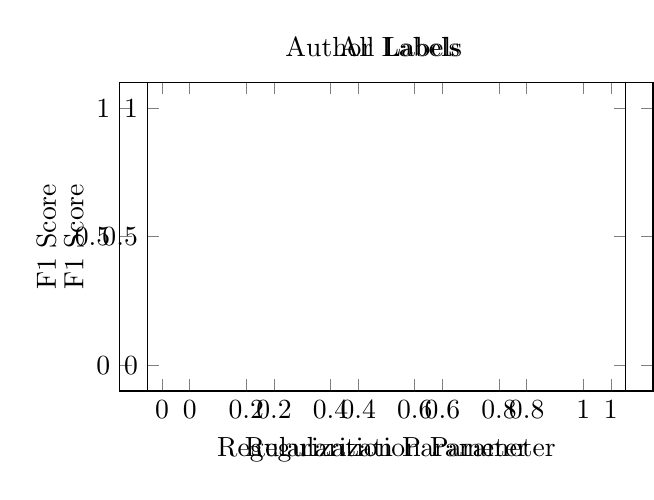
\begin{tikzpicture}
\begin{axis}[
    \firstchartconfig
    title={Author Labels},
    ylabel={F1 Score},
    \barchartconfig
    \colorlist
]
\plotfile{/home/martin/mt/plots/end-tags-labels-f1.dat}
\legend{}; % empty the legend
\end{axis}

\hskip 10pt

\begin{axis}[
    \secondchartconfig
    title={All Labels},
    ylabel={F1 Score},
    yticklabel style={/pgf/number format/precision=3},
    \barchartconfig
    \colorlist
]
\plotfile{/home/martin/mt/plots/end-tags-total-f1.dat}
\legend{}; % empty the legend
\end{axis}
\end{tikzpicture}
}
\vspace*{-\baselineskip}

\caption{Results for models using the \gls{bio} labeling in comparison to the \gls{bieo} labeling.}
\label{fig:eval-end-tags}
\end{figure}

\bigskip

\RQ{3} addresses how the probability mass is assigned to a \gls{ge} constraint for words $w_n$ that are matched to no author name.
For this, we compare two approaches.
The first one is to assign the full probability mass of $1$ to the label \texttt{O}.
In the second approach, we only assign a specified part of the probability mass to label \texttt{O}.
The remaining probability mass is then distributed over all other labels.
Instead of specifying this distribution for all other labels, we derive it from our distantly supervised training set.
For example, we assume that the label \texttt{B-FN} was used in $25\%$ of all author labels in the distantly supervised training set.
Further, we specify that $80\%$ of our probability mass is assigned to the label \texttt{O}.
Therefore, we assign $25\%$ of the remaining $20\%$ of the probability mass to the label \texttt{B-FN}.

The evaluation results are shown in \Cref{fig:eval-other-percentages}.
\begin{figure}
\pgfplotsset{xlabel={Probability Mass of \texttt{O} Label}}
\pgfplotsset{height=5.5cm,width=8cm}

\resizebox{\textwidth}{!}{%
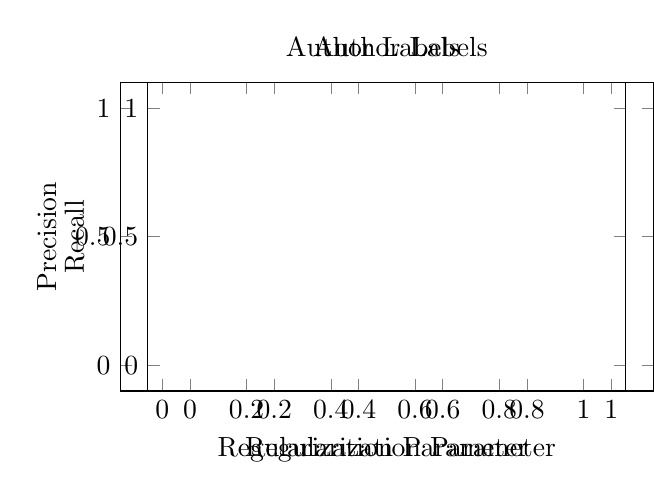
\begin{tikzpicture}
\begin{axis}[
    \firstchartconfig
    title={Author Labels},
    ylabel={Precision},
    yticklabel style={/pgf/number format/precision=3},
    \colorlist
]
\plotfile{/home/martin/mt/plots/other-percentages-labels-precision.dat}
\legend{}; % empty the legend
\end{axis}

\hskip 10pt

\begin{axis}[
    \secondchartconfig
    \secondchartlegendconfig
    legend style={font=\rmfamily},
    title={Author Labels},
    ylabel={Recall},
    yticklabel style={/pgf/number format/precision=3},
    \colorlist
]
\plotfile{/home/martin/mt/plots/other-percentages-labels-recall.dat}
\end{axis}
\end{tikzpicture}
}

\vspace{10pt}

\resizebox{\textwidth}{!}{%
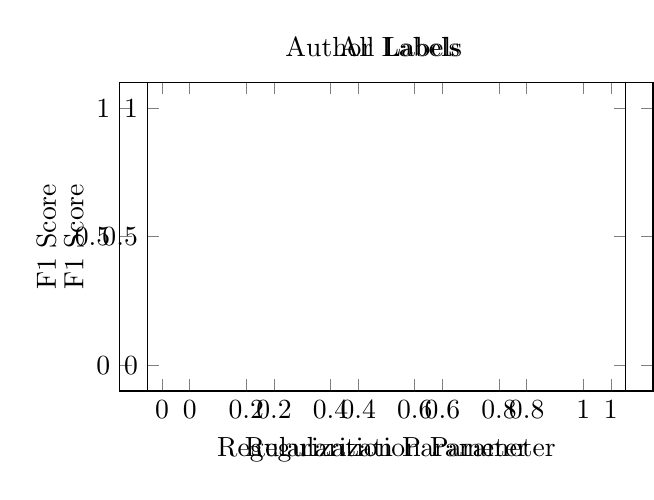
\begin{tikzpicture}
\begin{axis}[
    \firstchartconfig
    title={Author Labels},
    ylabel={F1 Score},
    \colorlist
]
\plotfile{/home/martin/mt/plots/other-percentages-labels-f1.dat}
\legend{}; % empty the legend
\end{axis}

\hskip 10pt

\begin{axis}[
    \secondchartconfig
    title={All Labels},
    ylabel={F1 Score},
    yticklabel style={/pgf/number format/precision=3},
    \colorlist
]
\plotfile{/home/martin/mt/plots/other-percentages-total-f1.dat}
\legend{}; % empty the legend
\end{axis}
\end{tikzpicture}
}
\vspace*{-\baselineskip}

\caption{Results for different probability masses assigned to the \texttt{O} label for building \gls{ge} constraints using the \texttt{swp-full} data set. 500, 1000, and 1500 are the number of used reference sections.}
\label{fig:eval-other-percentages}
\end{figure}
They suggest that increasing the probability mass of the \texttt{O} label also increases the \gls{precision} of the author labels but decreases their \gls{recall}.
As a result, this could provide a way of influencing the trade-off between the two metrics.
When considering the \gls{f1 score}, a probability mass of \texttt{O} of around 0.9 shows the best results considering both author labels and all labels.

\bigskip

\RQ{4} is focused on the ratio between matched and unmatched $w_n$ that are considered for building \gls{ge} constraints.
\Cref{tab:ssoar-number-of-tags} shows the number of \texttt{AU} nodes in the resulting \glspl{goddag} based on different knowledge bases.
\begin{table}
\centering
\begin{tabular}{l c c c c c}
 \toprule
\begin{tabular}[c]{@{}c@{}}Count\\Description\end{tabular} & \texttt{gnd-full} & \texttt{gnd-diff} &\texttt{swp-trim} &\texttt{swp-full} & \begin{tabular}[c]{@{}c@{}}\texttt{gnd-full}\\+\texttt{swp-full}\end{tabular} \\
 \midrule
 \texttt{AU} Nodes      & \num{1161744} &  \hphantom{1,}\num{958720}  & \hphantom{1,}\num{998163}  & \num{1203040} & \num{1407053}\\
 \texttt{AU} as Parent  & \num{1763518} &  \num{1553250} & \num{1729806} & \num{1959727} & \num{2084520}\\
 \bottomrule
\end{tabular}
\caption{Number of \texttt{AU} nodes and number of leaf nodes with at least one \texttt{AU} node as parent over all reference section \glspl{goddag}. Total number of leaf nodes: \num{17294919}.}
\label{tab:ssoar-number-of-tags}
\end{table}
Further, it shows the number of nodes that have at least on \texttt{AU} as a parent and thereby the number of words that are matches to at least one author.
Since only between $9\%$ and $12\%$ of the words are matched to an author, we investigate a balacing of the training set.

\Cref{fig:eval-other-ratios} summarizes the evaluation results for different percentages of unmatched words for the \gls{ge} constraints generation.
\begin{figure}
\pgfplotsset{xlabel={\#Unmatched Words / \#Matched Words}}
\pgfplotsset{height=5.5cm,width=8cm}

\resizebox{\textwidth}{!}{%
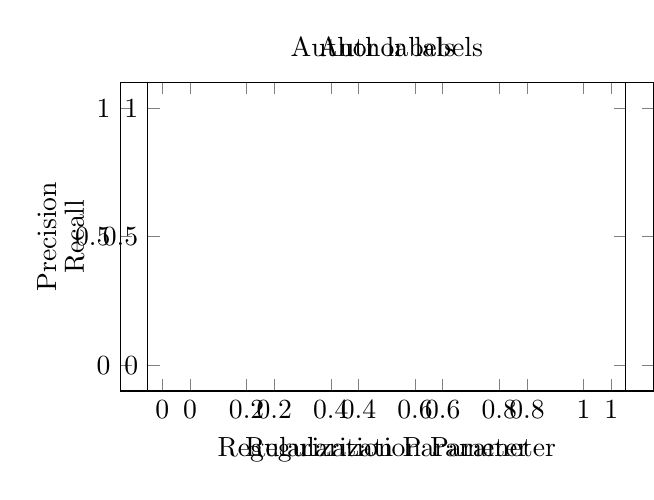
\begin{tikzpicture}
\begin{axis}[
    \firstchartconfig
    title={Author labels},
    ylabel={Precision},
    yticklabel style={/pgf/number format/precision=3},
    \colorlist
]
\plotfile{/home/martin/mt/plots/other-ratios-labels-precision.dat}
\legend{}; % empty the legend
\end{axis}

\hskip 10pt

\begin{axis}[
    \secondchartconfig
    \secondchartlegendconfig
    title={Author labels},
    ylabel={Recall},
    yticklabel style={/pgf/number format/precision=3},
    \colorlist
]
\plotfile{/home/martin/mt/plots/other-ratios-labels-recall.dat}
\end{axis}
\end{tikzpicture}
}

\vspace{10pt}

\resizebox{\textwidth}{!}{%
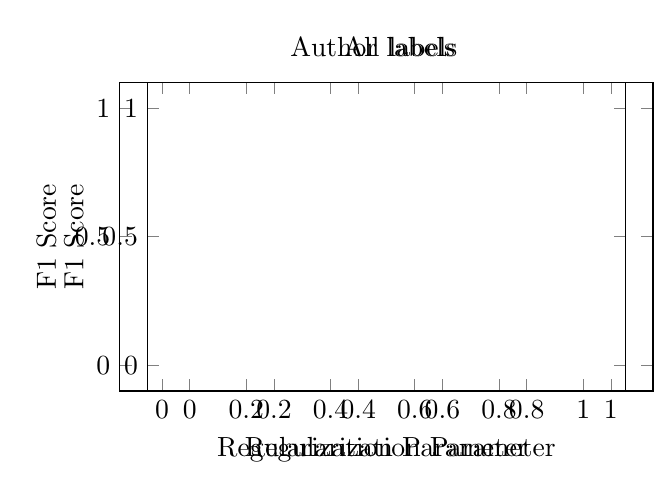
\begin{tikzpicture}
\begin{axis}[
    \firstchartconfig
    title={Author labels},
    ylabel={F1 Score},
    \colorlist
]
\plotfile{/home/martin/mt/plots/other-ratios-labels-f1.dat}
\legend{}; % empty the legend
\end{axis}

\hskip 10pt

\begin{axis}[
    \secondchartconfig
    title={All labels},
    ylabel={F1 Score},
    yticklabel style={/pgf/number format/precision=3},
    legend style={font=\ttfamily},
    \colorlist
]
\plotfile{/home/martin/mt/plots/other-ratios-total-f1.dat}
\legend{}; % empty the legend
\end{axis}
\end{tikzpicture}
}
\vspace*{-\baselineskip}

\caption{Results for different percentages of unmatched words for building \gls{ge} constraints using the \texttt{swp-full} data set. The number of matched words is fixed. 500, 1000, and 1500 are the number of used reference sections.}
\label{fig:eval-other-ratios}
\end{figure}
We can see that by increasing the percentage of unmatched words from $20\%$ to $69\%$, the \gls{recall} for author labels decreases by almost $10\%$.
At the same time, the \gls{precision} of author labels does not increase accordingly.
This is especially the case for the model that was learned with $1500$ reference sections.
When looking at the \glspl{f1 score}, we see for all three models that by increasing the percentage of unmatched words, the value first increases and then decreases.
The more reference sections were used, the lower is the percentage of unmatched words that results in the highest \glspl{f1 score}.

\bigskip

\RQ{5} considers a variation of the author extraction problem.
Instead of grouping words to individual author names and distinguishing between first and last names, a word $w_n$ is only labeled as part of an author name.
This results in a labeling which consists of two labels:
\texttt{A} for Author and \texttt{O} for Other.
We refer to this as the $\texttt{A-O}$ problem.

This can be addressed using our more fine-grained approach that includes the labels \texttt{B-FN}, \texttt{B-LN}, \texttt{I-FN}, \texttt{I-LN}, and \texttt{O}.
For this, we assume all labels except \texttt{O} to represent the \texttt{A} label.
Using the statistics from the fine-grained approach, we can derive the value of $FP(\texttt{A})$ with:
\begin{equation*}
\begin{split}
  FP(\texttt{A})&=true(\texttt{A})-FN(\texttt{A})\\
  &=total(\texttt{A})-FP(\texttt{O})\\
  &=total(\texttt{A})-(predicted(\texttt{O})-TP(\texttt{O})).\\
\end{split}
\end{equation*}
Here, $true(\texttt{A})$ refers to the number of words with label \texttt{A} in the manually labeled testing set and $predicted(\texttt{O})$ refers to the number of words with the label \texttt{O} that were predicted by the model.
Similarly, we can compute the value of $FN(\texttt{A})$.
This further allows us to compute $TP(\texttt{A})$ with:
\begin{equation*}
  TP(\texttt{A})=true(\texttt{A})-FP(\texttt{A}).
\end{equation*}
The values of $TP(\texttt{A})$, $FP(\texttt{A})$, and $FN(\texttt{A})$ are sufficient to calculate $precision(\texttt{A})$, $recall(\texttt{A})$, and $F1(\texttt{A})$.
We refer to this as the \texttt{A-O-deriv} labeling.

In comparison to this derivation, we also train separate models that only contain the two labels \texttt{A} and \texttt{O}.
The resulting labeling is referred to as \texttt{A-O-model}.

\Cref{fig:eval-authors-only} shows the performance of these two approaches for the $\texttt{A-O}$ problem.
\begin{figure}
\pgfplotsset{xlabel={Reference Sections in Training Set}}
\pgfplotsset{height=5.5cm,width=8cm}

\resizebox{\textwidth}{!}{%
\begin{tikzpicture}
\begin{axis}[
    \firstchartconfig
    title={Author Labels},
    ylabel={Precision},
    yticklabel style={/pgf/number format/precision=3},
    \barchartconfig
    \colorlist
]
\plotfile{/home/martin/mt/plots/authors-only-labels-precision.dat}
\legend{}; % empty the legend
\end{axis}

\hskip 10pt

\begin{axis}[
    \secondchartconfig
    \secondchartlegendconfig
    legend style={font=\ttfamily},
    title={Author Labels},
    ylabel={Recall},
    yticklabel style={/pgf/number format/precision=3},
    \barchartconfig
    \colorlist
]
\plotfile{/home/martin/mt/plots/authors-only-labels-recall.dat}
\end{axis}
\end{tikzpicture}
}

\vspace{10pt}

\resizebox{\textwidth}{!}{%
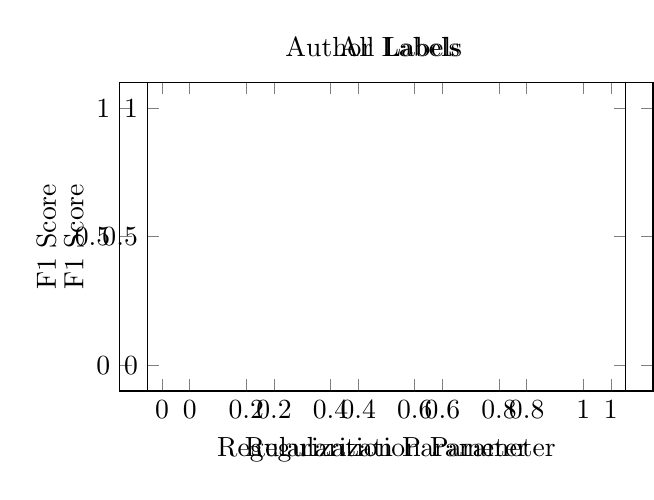
\begin{tikzpicture}
\begin{axis}[
    \firstchartconfig
    title={Author Labels},
    ylabel={F1 Score},
    \barchartconfig
    \colorlist
]
\plotfile{/home/martin/mt/plots/authors-only-labels-f1.dat}
\legend{}; % empty the legend
\end{axis}

\hskip 10pt

\begin{axis}[
    \secondchartconfig
    title={All Labels},
    ylabel={F1 Score},
    yticklabel style={/pgf/number format/precision=3},
    \barchartconfig
    \colorlist
]
\plotfile{/home/martin/mt/plots/authors-only-total-f1.dat}
\legend{}; % empty the legend
\end{axis}
\end{tikzpicture}
}
\vspace*{-\baselineskip}

\caption{Evaluation results that compare the \texttt{A-O-deriv} labeling with the \texttt{A-O-model} labeling for the \texttt{A-O} problem.}
\label{fig:eval-authors-only}
\end{figure}
The derived labeling consistently scores higher than the labeling by the model that was specifically trained for the \texttt{A-O} problem.
The latter also shows a stronger fluctuation in the result, depending on the randomly selected reference sections.
Yet, this result only gives a first intuition and should not be taken as an answer to \RQ{5}.
This is because we trained the model for the \texttt{A-O} problem using the same configuration as for the fine-grained model.
To come to a more conclusive answer, different configurations for the \texttt{A-O} model would need to be considered.

\bigskip

\RQ{6} focuses on the number of reference sections that are used in the unlabeled dataset $\mathcal{U}$ (see \Cref{subsec:generalized-expectation}).
Increasing the size of $\mathcal{U}$ also has an impact on the \gls{ge} constraints that are used in our model.
This is because the \gls{ge} constraints are generated from matched author names in $\mathcal{U}$ against the external list of author names.

To address the research question, we generate several models with a varying number of reference sections in $\mathcal{U}$.
\Cref{tab:eval-training-size} compares the models based on the metrics \gls{precision}, \gls{recall}, and \gls{f1 score} for the author labels and the \gls{f1 score} for all labels.
\begin{table}
\hspace{-0.25\textwidth}
\makebox[1.5\textwidth][c]{%
\begin{tabular}{c c r r r r r r r}
  \toprule
  Node Type &Metric & \multicolumn{1}{c}{\num{500}} & \multicolumn{1}{c}{\num{1000}} & \multicolumn{1}{c}{\num{1500}} & \multicolumn{1}{c}{\num{2000}} & \multicolumn{1}{c}{\num{2500}}  & \multicolumn{1}{c}{\num{5000}} & \multicolumn{1}{c}{\num{16470}}\\
  \midrule
  Author &\gls{precision} & $0.7845$ & $0.8328$ & $0.8471$ & $0.8593$ & $0.8473$ & $0.8336$ & $0.8349$ \\
  Author &\gls{recall}    & $0.8581$ & $0.8768$ & $0.9103$ & $0.9082$ & $0.9094$ & $0.9118$ & $0.9158$ \\
  Author &\gls{f1 score}  & $0.8197$ & $0.8542$ & $0.8776$ & $0.8831$ & $0.8773$ & $0.871$ & $0.8735$ \\
  All &\gls{f1 score}     & $0.9512$ & $0.9594$ & $0.9632$ & $0.9653$ & $0.9633$ & $0.9601$ & $0.9606$ \\
  \bottomrule
\end{tabular}
}
\caption{Comparison of models that use different numbers of reference sections for the model learning.}
\label{tab:eval-training-size}
\end{table}
We see that a bigger data set does not automatically lead to a better \gls{f1 score} for all labels or even the author labels alone.
Yet, increasing the number of reference sections does lead to an improved \gls{recall} of author labels.
Again, further experiments are needed to confirm this intuition since the same configuration was used for all models.

\bigskip

\RQ{7} takes the \gls{markov order} of \glspl{linear-chain crf} into consideration.
For this, we compare three different models:
\begin{itemize}
  \item \texttt{MO-0}: A \gls{markov order} zero \gls{linear-chain crf}.
  \item \texttt{MO-1}: A \gls{markov order} one \gls{linear-chain crf}.
  \item \texttt{MO-0-1}: A \gls{markov order} one \gls{linear-chain crf} with \gls{markov order} zero states (see \Cref{subsec:i-graph-construction}).
\end{itemize}
We compare the models for three different training set sizes while using the \texttt{swp-full} author data set for creating \gls{ge} constraints.
The results are presented in \Cref{fig:eval-markov-orders}.
\begin{figure}
\pgfplotsset{xlabel={Reference Sections in Training Set}}
\pgfplotsset{height=5.5cm,width=8cm}

\resizebox{\textwidth}{!}{%
\begin{tikzpicture}
\begin{axis}[
    \firstchartconfig
    title={Author Labels},
    ylabel={Precision},
    yticklabel style={/pgf/number format/precision=3},
    \barchartconfig
    \colorlist
]
\plotfile{/home/martin/mt/plots/markov-orders-labels-precision.dat}
\legend{}; % empty the legend
\end{axis}

\hskip 10pt

\begin{axis}[
    \secondchartconfig
    \secondchartlegendconfig
    legend style={font=\ttfamily},
    title={Author Labels},
    ylabel={Recall},
    yticklabel style={/pgf/number format/precision=3},
    \barchartconfig
    \colorlist
]
\plotfile{/home/martin/mt/plots/markov-orders-labels-recall.dat}
\end{axis}
\end{tikzpicture}
}

\vspace{10pt}

\resizebox{\textwidth}{!}{%
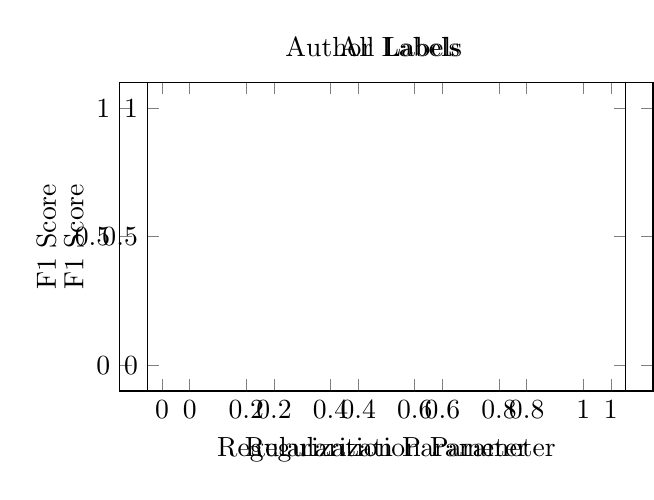
\begin{tikzpicture}
\begin{axis}[
    \firstchartconfig
    title={Author Labels},
    ylabel={F1 Score},
    \barchartconfig
    \colorlist
]
\plotfile{/home/martin/mt/plots/markov-orders-labels-f1.dat}
\legend{}; % empty the legend
\end{axis}

\hskip 10pt

\begin{axis}[
    \secondchartconfig
    title={All Labels},
    ylabel={F1 Score},
    yticklabel style={/pgf/number format/precision=3},
    \barchartconfig
    \colorlist
]
\plotfile{/home/martin/mt/plots/markov-orders-total-f1.dat}
\legend{}; % empty the legend
\end{axis}
\end{tikzpicture}
}
\vspace*{-\baselineskip}

\caption{Evaluation results that compare \glspl{linear-chain crf} of different \glspl{markov order} using the \texttt{swp-full} data set with for different numbers of reference sections.}
\label{fig:eval-markov-orders}
\end{figure}
They show that a \gls{markov order} zero model (\texttt{MO-0}) has a better \gls{recall} but a worse \gls{precision} than a \gls{markov order} one model (\texttt{MO-1}).
The combined \texttt{MO-0-1} model does not have a better recall than the \texttt{MO-0} model or a better precision than the \texttt{MO-1} model for the training set with \num{1000} reference sections.
Yet, it always has a better \gls{f1 score} than the individual models.

We did not consider higher \glspl{markov order} since they would not be applicable to larger training sets both in terms of hardware requirements and runtime using the current implementation.
Yet, especially for author names that consist of more than two words, a higher \gls{markov order} could lead to improvements.

\bigskip

\RQ{8} aims to compare the impact of different \gls{regularization parameter} of the \gls{gaussian prior} in a \gls{linear-chain crf} model.
Again, we use three different training set sizes and the \texttt{swp-full} author data set to compare nine different \glspl{regularization parameter} between $5$ and $45$.
\Cref{fig:eval-gaussian} shows the corresponding evaluation results.
\begin{figure}
\pgfplotsset{xlabel={Regularization Parameter}}
\pgfplotsset{height=5.5cm,width=8cm}

\resizebox{\textwidth}{!}{%
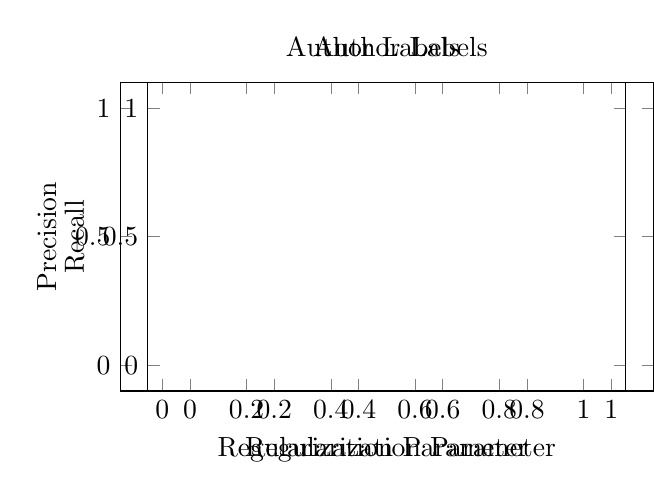
\begin{tikzpicture}
\begin{axis}[
    \firstchartconfig
    title={Author Labels},
    ylabel={Precision},
    yticklabel style={/pgf/number format/precision=3},
    \colorlist
]
\plotfile{/home/martin/mt/plots/gaussian-labels-precision.dat}
\legend{}; % empty the legend
\end{axis}

\hskip 10pt

\begin{axis}[
    \secondchartconfig
    \secondchartlegendconfig
    legend style={font=\rmfamily},
    title={Author Labels},
    ylabel={Recall},
    yticklabel style={/pgf/number format/precision=3},
    \colorlist
]
\plotfile{/home/martin/mt/plots/gaussian-labels-recall.dat}
\end{axis}
\end{tikzpicture}
}

\vspace{10pt}

\resizebox{\textwidth}{!}{%
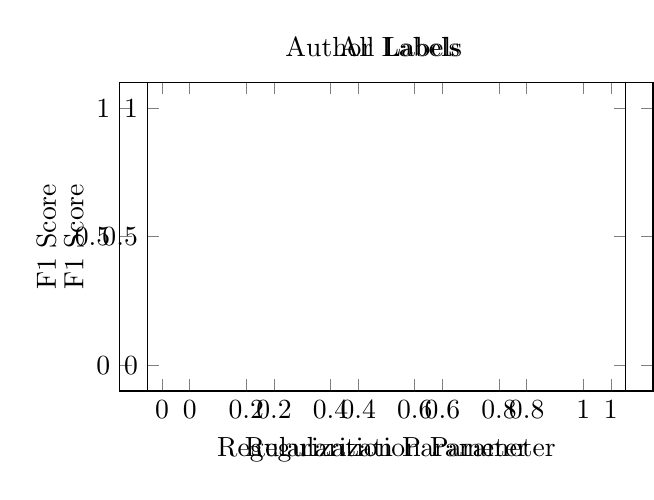
\begin{tikzpicture}
\begin{axis}[
    \firstchartconfig
    title={Author Labels},
    ylabel={F1 Score},
    \colorlist
]
\plotfile{/home/martin/mt/plots/gaussian-labels-f1.dat}
\legend{}; % empty the legend
\end{axis}

\hskip 10pt

\begin{axis}[
    \secondchartconfig
    title={All Labels},
    ylabel={F1 Score},
    yticklabel style={/pgf/number format/precision=3},
    \colorlist
]
\plotfile{/home/martin/mt/plots/gaussian-total-f1.dat}
\legend{}; % empty the legend
\end{axis}
\end{tikzpicture}
}
\vspace*{-\baselineskip}

\caption{Comparison of \glspl{linear-chain crf} with different \gls{markov order} using the \texttt{swp-full} data set with for different numbers of reference sections.}
\label{fig:eval-gaussian}
\end{figure}
They suggest that modifying the \gls{regularization parameter} in this range does not impact the performance to the resulting model.
This also confirms a similar statement by \citet{sutton2010introduction}.
Further experiments could investigate wider ranges for the \glspl{regularization parameter}.
In out other evaluations, we set this parameter to the value $10$.
According to \citet{sutton2010introduction}, this is a typical choice for training sets of a medium size.

%on gaussian prior: Additionally, \citet{sutton2010introduction} state that small changes to $\sigma^2$, for example up to a factor of 10, do not have a big impact on the accuracy of the final model.
%%sutton2010, page48: gauss=10 is typical for medium-sized training sets

\bigskip


In \Cref{app:learning-scalability}, we provide some insights on the scalability of our learning approach by comparing the main memory consumption as well as the runtime for different numbers of reference sections.

